%%%%%%%%%%%%%%%%%%%%%%%%%%%%%%%%%%%%%%%%%%%%%%%%%%%%%%%%%%%%%%%%%%%%%%%%%%%%%%%%%%%%%%%%%%%%%
%%									section 4.	Principe de Optimisation (α, \beta, \gamma)								%
%%%%%%%%%%%%%%%%%%%%%%%%%%%%%%%%%%%%%%%%%%%%%%%%%%%%%%%%%%%%%%%%%%%%%%%%%%%%%%%%%%%%%%%%%%%%%

\subsection{Principe d'Optimisation de $\alpha, \beta\; et\; \gamma$}
 
Dans le cadre du model checking, les états présentent des informations par rapport à la vérification. L’analyse de ces résultats, montre que la distribution des états fortement liés augmente le temps de traitement de la vérification. A titre d'exemple sur l'exemple précédente, la distribution des états $S1$ et $S5$ a augmenté le temps de la vérification du model checking car ces états sont liés. Dans un exemple plus complexe o\`{u} un ensemble d’états liés sont distribués, le temps de la vérification sera très élevé. Pour avoir une distribution de l'espace d'états respectant les objectifs fixés nous optimisons les paramètres $\alpha, \beta \; et\; \gamma$ en simulant un jeu non coopératif entre les machines. L'optimisation de ces paramètres est faite comme suit:
\begin{itemize}
	\item Sur Chaque machine on recherche le nombre d'états liés à chaque état sur lequel la formule n'est pa vérifiée, le paramètre $\beta$ pour cet état est égale à ce nombre. Les états local qui disposent des prédécesseurs directs sur d'autres machines distantes, la valeurs du paramètre correspond aux nombres des successeurs directs et indirects liés au même états.
	\item La limite des états liés ou dépendant peut entraîner la duplication de certain états, ce nombre états correspond à la valeur du paramètre $\gamma$. 
	\item En appliquant une heuristique sur les paramètres $\beta \; et\; \gamma$ de deux machines qui sont liées par un état nous obtenons une optimisation du paramètre $\alpha$.
\end{itemize}
Dans les sections suivantes, nous détaillons les phases de ce principe d'optimisation, la structure de Kripke présentée sur la Figure \ref{skd2} sera utilisée dans les exemples. \\

A partir du nombre d'états stockés dans chaque machine il est possible de calculer le nombre minimum et maximum d’états susceptibles d’être stockés par deux machine. Le calcul de cet interval est comme suit :

\begin{itemize}
	\item  	Soit $(\beta1 \; et\; \gamma1)$ les valeurs de la machine $M_1$ respectivement pour la machine $M_2$ $(\beta2 \;et\; \gamma2)$.
	\item  	$\overline{\beta}$ la moyenne des états $\overline{\beta}=\frac{\beta1+\beta2}{2}$.
	\item  	L’écart type $\delta=\sqrt{\frac{\displaystyle\sum_{i=1}^{2}\beta_i^2 }{2}-\overline{\beta}^2} $
\end{itemize}
 
	\begin{center}
		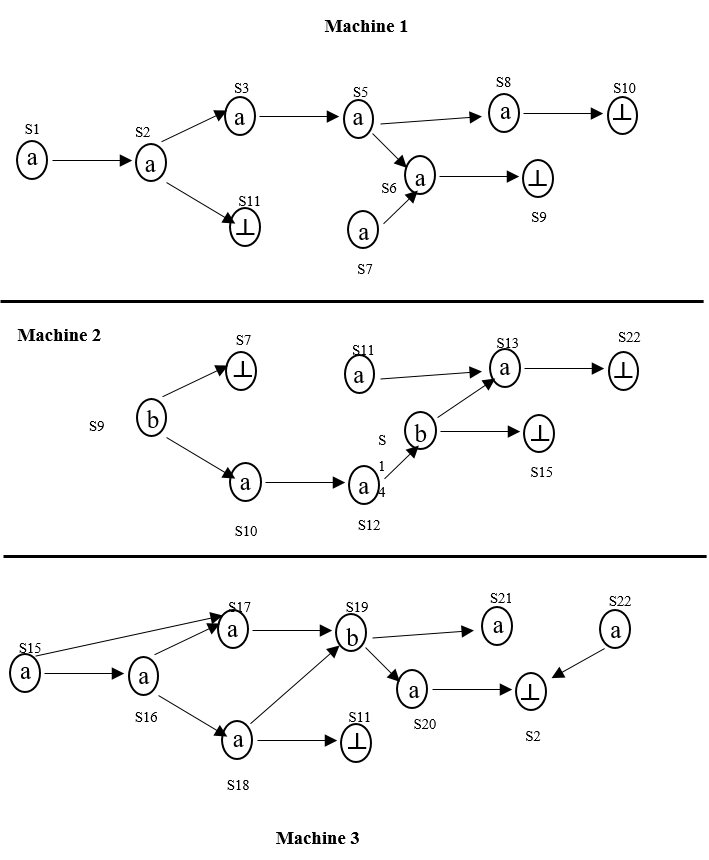
\includegraphics[height=4in]{img/skd2.png}	
	\captionof{figure}{Structure de Kripke distribu\'{e}} \label{skd2}
	\end{center}

